% TODO famous example for a product line failure?

\subsection{Recap: Software Testing}
\begin{frame}{\myframetitle{}}
	\begin{mycolumns}
		\uncover<1->{
			\begin{definition}{Software Testing \mysource{\sommerville}}
				\mycite{Testing is intended to show that a program does what it is intended to do and to discover program defects before it is put into use.}
			\end{definition}
		}
		\uncover<2->{
			\begin{definition}{Validation Testing \mysource{\sommerville}}
				\mycite{Demonstrate to the developer and the customer that the software meets its requirements.}
			\end{definition}
		}
		\uncover<3->{
			\begin{definition}{Defect Testing \mysource{\sommerville}}
				\mycite{Find inputs or input sequences where the behavior of the software is incorrect, undesirable, or does not conform to its specification.}
			\end{definition}
		}
	\mynextcolumn
		\uncover<4->{
			\begin{note}{Stages of Testing \mysource{\sommerville}}
				\begin{itemize}
					\setlength\itemsep{.1em}
					\item[1.] \mycite{\emph{Development testing}, where the system is tested during development to discover
					bugs and defects}
					\item[2.] \mycite{\emph{Release testing}, where a separate testing team tests a complete version of the
					system before it is released to users}
					\item[3.] \mycite{\emph{User testing}, where users or potential users of a system test the system in their
					own environment}
				\end{itemize}
			\end{note}
		}
		\uncover<5->{
			\begin{note}{Manual vs Automated Testing \mysource{\sommerville}}
				\mycite{In \emph{manual testing}, a tester runs the program with some test data and
				compares the results to their expectations. [...] In \emph{automated testing}, the tests are encoded in a program that is run each time the system under development is to be tested.}
			\end{note}
		}
	\end{mycolumns}
\end{frame}

\subsection{Test-Case Design in Single-System Engineering}
\begin{frame}{Recap: Test-Case Design \deutschertitel{Testfallentwurf}}
	\begin{mycolumns}
		\begin{definition}{Systematic Test \mysource{\ludewiglichter}}
			A systematic test is a test, in which
			\begin{itemize}
				\setlength\itemsep{.1em}
				\item[1.] the \emph{setup} is defined,
				\item[2.] the \emph{inputs} are chosen systematically,
				\item[3.] the \emph{results} are documented and evaluated by criteria being defined prior to the test. 
			\end{itemize}
		\end{definition}
		\pause
		\begin{definition}{Test Case \mysource{\ludewiglichter}}
			In a test, a number of test cases are executed, whereas each test case consists \emph{input values} for a single execution and \emph{expected outputs}. An \emph{exhaustive test} refers a test in which the test cases exercise all the possible inputs.
		\end{definition}
	\mynextcolumn
		\pause
		\begin{note}{Goal \mysource{\ludewiglichter}}%
			Detect a large number of failures with a low number of test cases. A test case (execution) is \emph{positive}, if it detects a failure, and \emph{successful} if it detects an unknown failure.
		\end{note}
		\pause
		\begin{definition}{An ideal test case is \ldots \mysource{\ludewiglichter}}
			\begin{itemize}
				\setlength\itemsep{.1em}
				\item representative: represents a large number of feasible test cases
				\item failure sensitive: has a high probability to detect a failure
				\item non-redundant: does not check what other test cases already check
			\end{itemize}
		\end{definition}
	\end{mycolumns}
\end{frame}

% TODO recap analysis strategies for product lines and discuss why feature based and family based is typically not feasible for testing

\subsection{Testing All Configurations}
\begin{frame}{\myframetitle{}}
	\begin{mycolumns}[forget]
		\centering\featureDiagramConfigurableDatabase
		
		\begin{example}{Recap: 26 Valid Configurations\mysource{\lecturemodeling}}
			\footnotesize
			\begin{mycolumns}[animation=none]
				$\{C,G,W\}$\\
				$\{C,P,W\}$\\
				$\{C,G,P,W\}$\\
				$\{C,D,W\}$\\
				$\{C,G,D,W\}$\\
				$\{C,P,D,W\}$\\
				$\{C,G,P,D,W\}$\\
				$\{C,P,T,W\}$\\
				$\{C,G,P,T,W\}$\\
				$\{C,D,T,W\}$\\
				$\{C,G,D,T,W\}$\\
				$\{C,P,D,T,W\}$\\
				$\{C,G,P,D,T,W\}$
			\mynextcolumn
				$\{C,G,L\}$\\
				$\{C,P,L\}$\\
				$\{C,G,P,L\}$\\
				$\{C,D,L\}$\\
				$\{C,G,D,L\}$\\
				$\{C,P,D,L\}$\\
				$\{C,G,P,D,L\}$\\
				$\{C,P,T,L\}$\\
				$\{C,G,P,T,L\}$\\
				$\{C,D,T,L\}$\\
				$\{C,G,D,T,L\}$\\
				$\{C,P,D,T,L\}$\\
				$\{C,G,P,D,T,L\}$
			\end{mycolumns}
		\end{example}
	\mynextcolumn
		\vspace{-7mm}
		\begin{note}{Discussion}
			\begin{itemize}
				\setlength\itemsep{.5em}
				\item only feasible for \emph{small} product lines\\(few valid configurations)
				\item redundant test effort
				\vspace*{1ex}
				\item large product lines: not feasible to generate and compile all configurations
				\begin{itemize}
					\item (some) large product lines: even number of valid configurations is unknown
				\end{itemize}
			\end{itemize}
		\end{note}
	\end{mycolumns}
\end{frame}

\begin{frame}{Recap: Feature Model of the Linux Kernel}
	\vspace{1mm}~\hspace{-15mm}\href{https://dl.acm.org/doi/abs/10.1145/3382025.3414943}{\includegraphics[width=1.2\linewidth,page=1,trim=100 510 100 170,clip]{2020/2020-SPLC-Thuem}}
\end{frame}

\begin{frame}{\myframetitle{}}
	\begin{mycolumns}[widths={60}]
		\begin{exampletight}{Recap: Industrial Configuration Spaces\mysource{\lectureintroduction}}
			\centering\evaluatingsharpsatsolverslink{\includegraphics[width=\linewidth,page=6,trim=50 210 320 440,clip]{2020/2020-VaMoS-Sundermann}}
		\end{exampletight}
		\uncover<3->{
			\begin{note}{}
				Why being complete on the configurations then?
			\end{note}
		}
	\mynextcolumn
		\vspace{-7mm}
		\href{https://commons.wikimedia.org/wiki/File:Edsger_Wybe_Dijkstra.jpg}{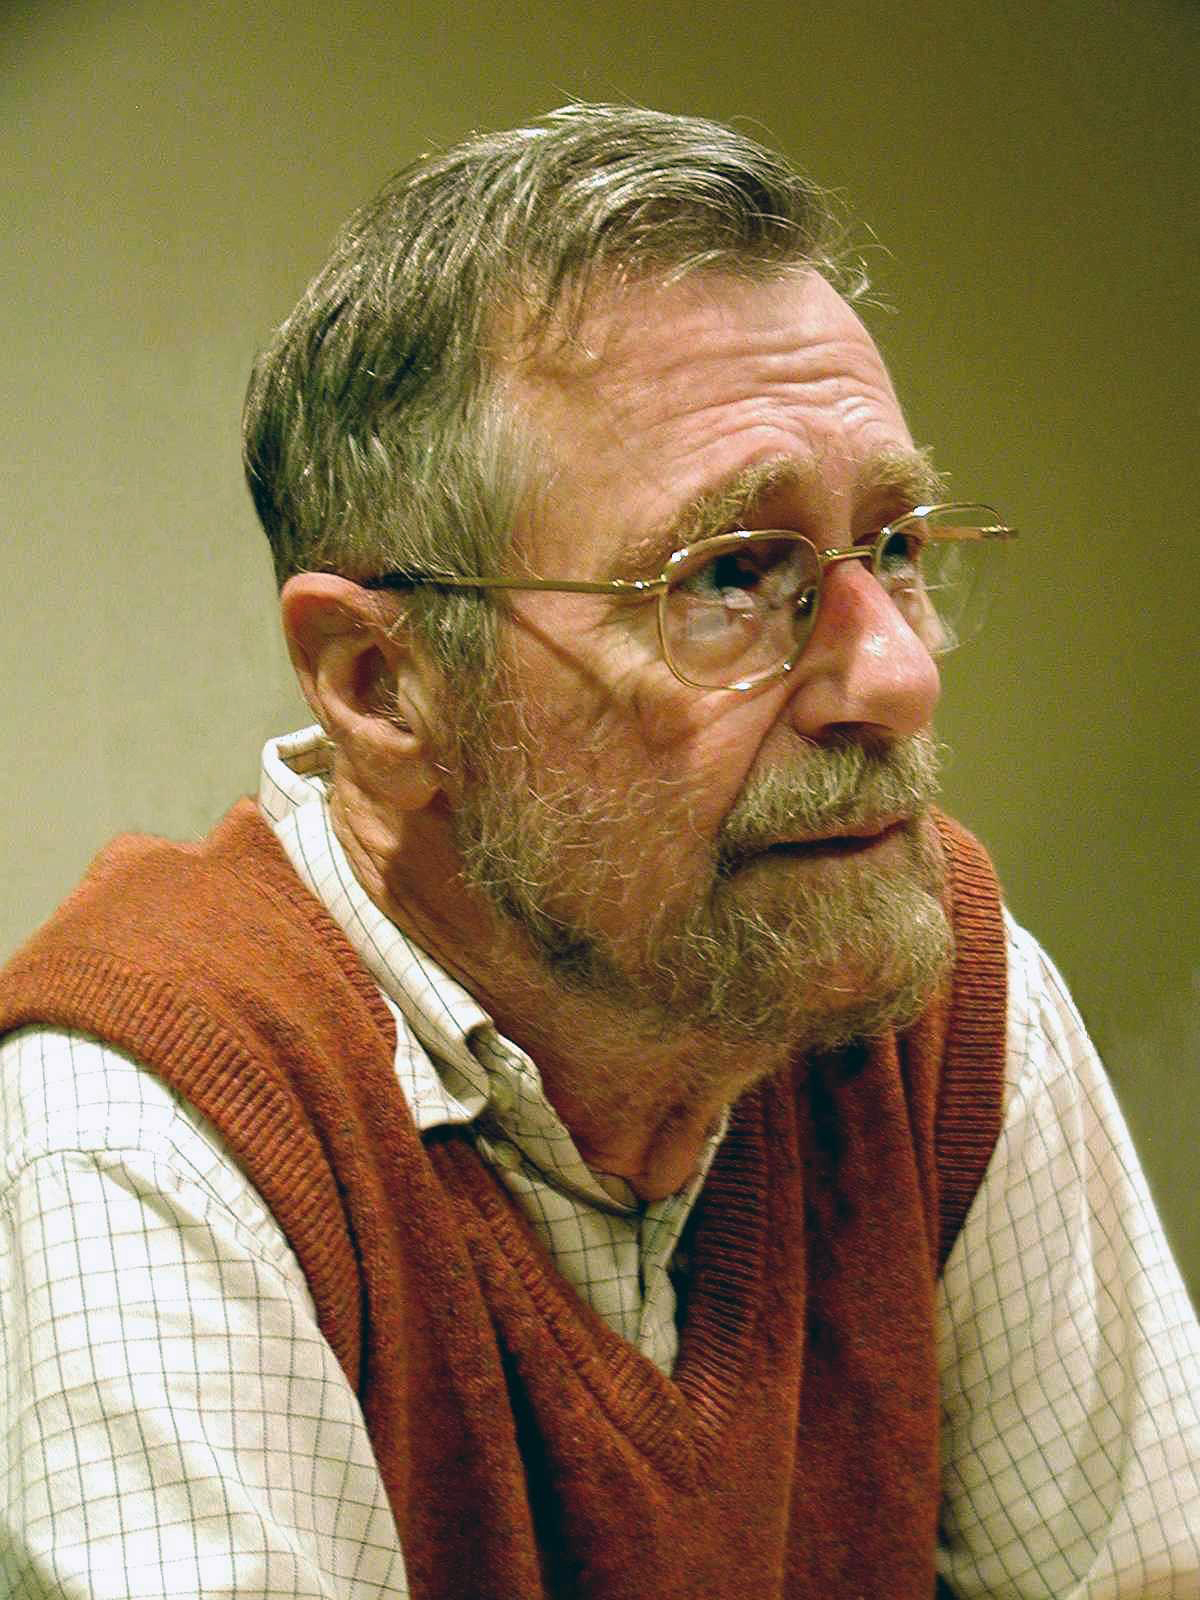
\includegraphics[width=\linewidth,trim=0 425 0 75,clip]{edsger-dijkstra}}
		\vspace{-7mm}
		
		\begin{note}{Edsger W. Dijkstra (1972)}
			\mycite{Program testing can be a very effective way to show the presence of bugs, but it is hopelessly inadequate for showing their absence.}\mysource{\thehumbleprogrammer}
		\end{note}
		% 1930-2002, ACM Turing Award winner
	\end{mycolumns}
\end{frame}

\newcommand{\eemph}[1]{{\color{red}\textbf{#1}}}

\subsection{Testing One Configuration}
\begin{frame}[b]{\myframetitle{}}
	\begin{mycolumns}[b]
		\centering\featureDiagramConfigurableDatabase
		
		\begin{example}{Recap: 26 Valid Configurations\mysource{\lecturemodeling}}
			\footnotesize
			\begin{mycolumns}[animation=none]
				$\{C,G,W\}$\\
				$\{C,P,W\}$\\
				$\{C,G,P,W\}$\\
				$\{C,D,W\}$\\
				$\{C,G,D,W\}$\\
				$\{C,P,D,W\}$\\
				$\{C,G,P,D,W\}$\\
				$\{C,P,T,W\}$\\
				$\{C,G,P,T,W\}$\\
				$\{C,D,T,W\}$\\
				$\{C,G,D,T,W\}$\\
				$\{C,P,D,T,W\}$\\
				\emph{$\{C,G,P,D,T,W\}$}
			\mynextcolumn
				$\{C,G,L\}$\\
				$\{C,P,L\}$\\
				$\{C,G,P,L\}$\\
				$\{C,D,L\}$\\
				$\{C,G,D,L\}$\\
				$\{C,P,D,L\}$\\
				$\{C,G,P,D,L\}$\\
				$\{C,P,T,L\}$\\
				$\{C,G,P,T,L\}$\\
				$\{C,D,T,L\}$\\
				$\{C,G,D,T,L\}$\\
				$\{C,P,D,T,L\}$\\
				$\{C,G,P,D,T,L\}$
			\end{mycolumns}
		\end{example}
	\mynextcolumn
		\pause\vspace{-10mm}
		\begin{note}{Discussion}
			\begin{itemize}
				\setlength\itemsep{.4em}
				\item applicable to large product lines
				\item strategy in practice: all-yes-config (configuration with many features selected)
				\item no redundant test effort (from configurations)
				\vspace*{1ex}
				\item often unfeasible to test all features wit a single configuration (e.g., \texttt{Windows} and \texttt{Linux})
				\item[$\Rightarrow$] unnoticed feature interactions\mysource{\lectureinteractions}
			\end{itemize}
		\end{note}
		\pause
		\begin{example}{What about interactions with missing features?}
			\centering\pic[width=.5\linewidth]{toast4}
		\end{example}
	\end{mycolumns}
\end{frame}

\subsection{Sample-Based Testing}
\begin{frame}{\myframetitle{} \deutschertitel{Stichprobenbasiertes Testen}}
	\begin{mycolumns}
		\begin{definition}{Intuition}
			\begin{itemize}
				\item to analyze the product line, just analyze \emph{some products}
				\item sample \deutsch{Stichprobe} refers to a subset of all valid configurations
				\item common technique to test a product line
				\item sample configurations chosen by experts, randomly, or systematically
			\end{itemize}
		\end{definition}
		\pause
		\begin{note}{Advantages and Challenges}
			\begin{itemize}
				\item[+] lower effort than testing all configurations
				\item[+] higher chance to detect defects than testing one configuration
				\item[--] how many configurations to test?\\which configurations to test?
			\end{itemize}
		\end{note}
	\mynextcolumn
		\pause
		\pic[width=\linewidth,page=10]{lego-analyses}
	\end{mycolumns}
\end{frame}

% TODO \subsection{Expert Knowledge in Sampling}

% TODO \subsection{Random Sampling}

% TODO probably too much content anyway: \subsection{Excursus: Uniform Random Sampling}

% TODO \subsection{Testing the Linux Kernel}
% allyesconfig

%\subsection{Automation in Product Sampling} ???

%\subsection{Missing: Test-Case Selection/Generation}
% What to test for those configurations? Variable unit tests? Avoid redundant testing?

% TODO how Linux is developed: patches on mailing list, only considered if not rejected by CI, what happens in CI

